\documentclass{article}[12pt]

%----- Math ---------------------------------------------
\usepackage{amsmath}   
\usepackage{mathrsfs}      
\usepackage{mathtools}       
\usepackage{amssymb}   
\usepackage{amsthm}   
\usepackage{esint}     
\usepackage{resmes} 
\usepackage{stackengine}
\usepackage{amsfonts}
\usepackage{stmaryrd}
\usepackage{dsfont}



%----- Design ------------------------------------------- 
\usepackage{lastpage}                              
\usepackage{enumitem}
\usepackage{multirow}


%----- Intestazioni ---------------------------------------
\usepackage{fancyhdr}
\pagestyle{fancy}
\fancyhf{} % Clear all headers and footers
\fancyhead[R]{\nouppercase{\leftmark}} % Header right on all pages
\fancyfoot[C]{\thepage} % Footer center, page number
\setlength{\headheight}{14.5pt}

% Pacchetto titlesec per personalizzare i titoli dei capitoli
\usepackage{titlesec}


%----- Pacchetti Disegno --------------------------------
\usepackage{tikz}
\makeatother 
\usetikzlibrary{3d,perspective}
\usetikzlibrary{patterns}
\usetikzlibrary{arrows,calc,patterns}
\usepackage{tikz-cd}
\usepackage{graphicx}
\usepackage{thmtools}
\usepackage{xcolor}
\usepackage[all]{xy}        
\usetikzlibrary{decorations.markings}
\usetikzlibrary{hobby}
\usepackage{pgfplots}
\pgfplotsset{compat=1.18}


%----- Symbols -----------------------------------------
% ------ CAPITAL MATHBB --------------------
\providecommand{\B}{\mathbb{B}}
\providecommand{\C}{\mathbb{C}}
\providecommand{\D}{\mathbb{D}}
\providecommand{\E}{\mathbb{E}}
\providecommand{\F}{\mathbb{F}}
\providecommand{\M}{\mathbb{M}}
\providecommand{\N}{\mathbb{N}}
\providecommand{\Pbb}{\mathbb{P}}
\providecommand{\Q}{\mathbb{Q}}
\providecommand{\R}{\mathbb{R}}
\providecommand{\Sp}{\mathbb{S}}
\providecommand{\T}{\mathbb{T}}
\providecommand{\Z}{\mathbb{Z}}

%------- CAPITAL MATHCAL --------
\providecommand{\Tcal}{\mathcal{T}}
\providecommand{\Lcal}{\mathcal{L}}
\providecommand{\Mcal}{\mathcal{M}}
\providecommand{\Acal}{\mathcal{A}}


%-------- GREEK -----------
\providecommand{\eps}{\varepsilon}
\providecommand{\vp}{\varphi}

%-------- STANDARD MATH ---------
\providecommand{\Fam}{\mathscr{F}}
\providecommand{\id}{\mathrm{id}}
\providecommand{\Id}{\mathrm{Id}}
\providecommand{\obar}[1]{\overline{#1}}
\DeclareMathOperator{\re}{Re}
\DeclareMathOperator{\im}{Im}
\DeclareMathOperator{\val}{val}
\DeclareMathOperator{\Ind}{Ind}
\DeclareMathOperator{\ind}{ind}
\DeclareMathOperator{\codim}{codim}


%-------- ARROWS ---------
\providecommand{\mapsfrom}{\mathrel{\reflectbox{\ensuremath{\mapsto}}}}
\providecommand{\weakto}{\rightharpoonup}
\providecommand{\weakstarto}{\mathrel{\ensurestackMath{\stackon[1pt]{\rightharpoonup}{\scriptstyle\ast}}}}


%-------- CALCULUS ----------------
\providecommand{\de}{\partial}
\providecommand{\dif}{\mathrm{d}}
\providecommand{\acosh}{\mathrm{cosh}^{-1}}
\DeclareMathOperator{\dist}{dist}
\DeclareMathOperator{\diam}{diam}
\DeclareMathOperator{\gr}{graph}
\DeclareMathOperator{\dive}{div}
\DeclareMathOperator{\supp}{supp}
\DeclareMathOperator{\spt}{spt}
\DeclareMathOperator{\Conv}{Conv}
\DeclareMathOperator{\Hess}{Hess}
\DeclareMathOperator{\grad}{grad}
\DeclareMathOperator{\Crit}{Crit}
\DeclareMathOperator{\Reg}{Reg}

%--------- TOPOLOGY ---------
\DeclareMathOperator{\ext}{ext}
\DeclareMathOperator{\inte}{int}
\providecommand{\clos}[1]{\overline{#1}}

%--------- ALGEBRA ------
\DeclareMathOperator{\End}{End}
\DeclareMathOperator{\Hom}{Hom}
\DeclareMathOperator{\rank}{rank}
\DeclareMathOperator{\tr}{tr}
\DeclareMathOperator{\trace}{trace}
\DeclareMathOperator{\Span}{Span}
\DeclareMathOperator{\coker}{coker}

%-------- DIFFERENTIAL GEOMETRY ----
\providecommand{\sff}{\mathrm{I\!I}}
\DeclareMathOperator{\area}{area}
\DeclareMathOperator{\Area}{Area}
\DeclareMathOperator{\len}{length}
\DeclareMathOperator{\Len}{Length}
\DeclareMathOperator{\Ric}{Ric}
\DeclareMathOperator{\Rm}{Rm}
\DeclareMathOperator{\Sec}{Sec}
\DeclareMathOperator{\Scal}{Scal}
\DeclareMathOperator{\Rscal}{R}
\providecommand{\VF}{\mathfrak{X}}

%--------- MEASURE THEORY -----------
\providecommand{\Haus}{\mathscr{H}}
\providecommand{\Leb}{\mathscr{L}}
\usepackage{resmes}
\DeclareMathOperator{\essup}{essup}
\DeclareMathOperator{\Sing}{Sing}

%----- Hyperref ------------------------------------------
\usepackage{nameref}
\usepackage{csquotes}
\usepackage{hyperref}
\hypersetup{
	colorlinks=true,
	linkcolor=black, % Color for normal internal links
	filecolor=black, % Color for file links
	urlcolor=blue, % Color for external links
	citecolor=blue % Color for citations
}
\usepackage{cleveref} 


% -----Ambienti matematici-------------------------------
\theoremstyle{plain}
\newtheorem{thm}{Theorem}[section]
\newtheorem*{thm*}{Theorem}
\newtheorem{prop}[thm]{Proposition}
\newtheorem{cor}[thm]{Corollary}
\newtheorem{lemma}[thm]{Lemma}
\newtheorem{claim}{Claim}

\theoremstyle{definition}
\newtheorem{defn}[thm]{Definition}
\newtheorem{axiom}{Axiom}

\theoremstyle{remark}
\newtheorem{rmk}[thm]{Remark}
\newtheorem{ex}[thm]{Example}
\newtheorem{exercise}{Exercise}


%------BIBLIOGRAFIA-----------
\usepackage[style=alphabetic, backend=biber]{biblatex}
% Definizione di un nuovo driver per nascondere URL e DOI
\AtEveryBibitem{
 	\clearfield{url} % Nasconde l'URL
 	\clearfield{doi} % Nasconde il DOI
 	\clearfield{isbn} % Nasconde ISBN
 	\clearfield{issn} % Nasconde ISSN
 	\clearfield{note} % Nasconde le note
}
\addbibresource{biblio.bib}

\title{The isoperimetric inequality}
\author{Andrea Martelli}
\date{Trento, November 2025}
\begin{document}

\maketitle

\begin{abstract}
    These notes are the content of my seminar for the final exam of the course \emph{Advanced Topics in Analysis}, taught by Prof. Gian Paolo Leonardi during the Fall semester of 2025 at University of Trento.
\end{abstract}
%\tableofcontents

\section{Introduction}
In these notes we are going to prove the isoperimetric inequality, characterizing the equality case. The main reference is \cite[\S13.2 and Chapter~14]{Maggi_2012}.

\begin{thm}[Isoperimetric inequality]\label{thm: isoperimetric inequality}
    For every Lebesgue measurable set \(E \subset \R^n\),
    \[
        P(E) \ge n \omega_n^{1/n} |E|^{\frac{n-1}{n}},
    \]
    where \(\omega_n = |B_1|\) is the \(n\)-volume of the standard unit ball of \(\R^n\). Moreover, the equality holds if and only if \(E\) is equivalent to a ball, meaning that there exist \(x \in \R^n\) and \(R>0\) (that necessarily satisfies \(|E|=\omega_nR^n\)) such that \(|E \triangle B_R(x)|=0\).
\end{thm}
In other words, we prove that for every \(R>0\)
\[
    \inf \{ P(E) \colon E \subset \R^n, |E|=\omega_n R^n\} = n \omega_n R^{n-1}
\]
and it is realized only by sets equivalent to balls of radius \(R\).

When \(n=1\), this is quite easy.

\begin{thm}[1-dimensional isoperimetric inequality]\label{thm: 1D isoperimetric inequality}
    If \(E \subset \R\) is a Lebesgue measurable set with \(|E|<\infty\), then
    \[
        P(E)\ge 2,
    \]
    with equality if and only if \(E\) is equivalent to an interval of length \(|E|\).
\end{thm}
\begin{proof}
    Assume that \(P(E)<\infty\). Then \(E\) is equivalent to a finite union of disjoint open intervals, so \(P(E)=2N\) where \(N\) is the number of intervals.
\end{proof}

For \(n>1\), the proof of the inequality is not hard: on bounded sets it's just the direct method (cf. Lemma~\ref{lemma: constrained isoperimetric inequality}), and the unbounded case can be obtained by approximating finite perimeter sets with bounded finite perimeter sets. 

The actual work is to characterize the equality, i.e., minimizers of the variational problem
\begin{equation}\label{eq: isoperimetric problem with perimeter}
    \inf\{ P(E) \colon E \subset \R^n \text{ Lebesgue measurable}, |E|=m\},
\end{equation}
for \(m>0\) fixed.
A way to proceed is by using the Steiner inequality (cf. Theorem~\ref{thm: steiner inequality}), which states that the Steiner symmetrization does not increase the perimeter. This implies that minimizers must have many symmetries, and it's not hard to deduce that they are balls. Therefore, a sketch of the proof is to show, in order
\begin{itemize}
    \item finite perimeter sets can be approximated by bounded sets with polyhedral boundary (cf. Theorem~\ref{thm: polyhedral approximation});
    \item the Steiner inequality, proving it first on sets with polyhedral boundary and then approximating;
    \item minimizers of \eqref{eq: isoperimetric problem with perimeter} must be equivalent to balls, using the Steiner inequality.
\end{itemize}


Another approach that I find interesting is considering the problem from the point of view of differential geometry. Consider the class of smooth, connected, compact hypersurfaces that are the boundary of some open bounded set \(\Omega\). The critical points of the \((n-1)\)-area functional (i.e., the \((n-1)\)-Hausdorff measure restricted to the class of such hypersurfaces) with respect to volume preserving variations are called \emph{CMC} (because, by the first variation formula, they have constant mean curvature). Therefore, any minimizer of the variational problem
\[
\inf\left\{ \Haus^{n-1}(\Sigma) \left| \ \begin{aligned}
        &\Sigma = \de \Omega \text{ smooth, connected,}\\
        &\text{compact hypersurface}, |\Omega|=m
    \end{aligned}
    \right.\right\}.
\]
(for \(m>0\) fixed) must be CMC and must be stable with respect to volume preserving variations. However, Barbosa and do Carmo (\cite{BarbosaDoCarmo}, cf. Theorem~\ref{thm: Barbosa-do Carmo}) proved that the only smooth, connected, compact hypersurfaces of \(\R^n\) are the round spheres. The proof, sketched in the last section of these notes, is quite simple and exploits the stability inequality to prove that every CMC-stable hypersurface must be totally umbilical, hence, if it's connected, a sphere. 

\section{Polyhedral approximation}
Given a function \(u \colon \R^{n-1} \to \R\) and a subset \(G \subset \R^{n-1}\), we define the \emph{graph of \(u\) over \(G\)} as
\[
    \Gamma(u,G) \coloneq \{ (x,u(x)) \in \R^n \colon x \in G\}.
\]

\begin{defn}
    A \emph{polyhedral set} is a finite, non empty intersection of closed half-spaces.
    
    A continuous function \(u \colon G \subset \R^n \to \R\) is said to be \emph{finitely piecewise affine} if there exists a finite partition of polyhedral sets \(\{G_i\}_{i=1}^k\) of \(G\) such that \(u\) is affine on each \(G_i\).

    A set \(E\subset \R^n\) is said to have \emph{polyhedral boundary} if for every \(x \in \de E\) there exist \(r>0\), a finitely piecewise affine function \(u \colon (-r,r)^{n-1} \to \R\) and an isometry \(T \colon \R^n \to \R^n\) with \(T(x)=0\) such that
    \[
    \begin{aligned}
        T(\de E) \cap (-r,r)^n &= G(u,(-r,r)^{n-1})\\
        T(E) \cap (-r,r)^n &= \{ (z,t) \in (-r,r)^{n-1}\times (-r,r) \colon t>u(z) \}.
    \end{aligned}
    \]
\end{defn}
\begin{rmk}
    It's not hard to prove that any function \(u \in C^1_c(\R^n)\) can be approximated by \emph{compactly supported finitely piecewise affine functions} in the \(C^1\)-norm.
\end{rmk}

\begin{lemma}[Approximation by finitely piecewise affine functions]\label{lemma: approximation by finitely piecewise affine functions}
    For every \(u \in BV(\R^n)\) there exists a sequence \(u_h \colon \R^n \to \R\) of compactly supported finitely piecewise affine functions such that \(u_h \to u\) in the BV-strict sense, that is, \(u_h \to u\) in \(L^1(\R^n)\) and
    \[
        \int_{\R^n} |\nabla u_h| \dif z \to |Du|(\R^n).
    \]
\end{lemma}
\begin{proof}
    \emph{Step 1}. Assume that \(u \in C^1(\R^n) \cap BV(\R^n)\). Take a sequence of cutoff functions \(\varphi_h \colon \R^n \to \R\), that is, for some sequence \(R_h \nearrow \infty\), smooth functions with compact support in \(B_{R_h+1/h}\), \(0 \le \vp \le 1\) on \(\R^n\), \(\varphi_h = 1\) on \(B_{R_h}\) and \(\|\nabla \vp_h\|_{C^0} \le C\), \(C>0\) not depending on \(h\). Then \(v_h \coloneq u\vp_h \in C^1_c(\R^n)\), \(v_h \to u\) in \(L^1(\R^n)\), and
    \[
    \begin{aligned}
        \int_{\R^n} |\nabla v_h| \dif x &= \int_{B_{R_h}}|\nabla u| \dif x + \int_{B_{R_h+1/h}\setminus B_{R_h}} |\nabla v_h| \dif x \\
        &\to \int_{\R^n}|\nabla u| \dif x \qquad \text{ as }h \to \infty.
    \end{aligned}
    \]
    For every \(h \in \N\), take a sequence \(v_h^k \colon \R^n \to \R\) of compactly supported finitely piecewise affine functions approximating each \(v_h\) in \(C^1_c(\R^n)\) with respect to the \(C^1\)-norm. Then in particular \(v_h^k \to v_h\) in \(L^1(\R^n)\) and 
    \[
        \lim_{k\to \infty}\int_{\R^n} |\nabla v_h^k| \dif x = \int_{\R^n}|\nabla v_h|\dif x.
    \]
    With a diagonal argument, we can extract a diagonal sequence \(u_h \coloneq v_h^{k(h)}\) that satisfies the required properties.
    
    \emph{Step 2}. Now take any \(u \in BV(\R^n)\), and fix a kernel mollifier \(\rho \in C^\infty_c(\R^n)\). Let \(v_h = u \star \rho_{\eps_h}\), with \(\eps_h \to 0\), and for each \(h \in \N\) take a sequence \(v_h^k \colon \R^n \to \R\) of finitely piecewise affine functions approximating each \(v_h\), i.e., such that \(v_h^k \to v_h\) in \(L^1(\R^n)\) and
    \[
        \lim_{k\to \infty}\int_{\R^n} |\nabla v_h^k| \dif x = \int_{\R^n}|\nabla v_h|\dif x.
    \]
    By the properties of mollification,
    \[
        \lim_{h \to \infty} \int_{\R^n} |\nabla v_h| \dif x = |Du|(\R^n),
    \]
    so, as before, we can extract a diagonal sequence \(u_h \coloneq v_h^{k(h)}\) that satisfies the required properties.
\end{proof}

\begin{thm}[Polyhedral approximation]\label{thm: polyhedral approximation}
    Let \(E \subset \R^n\) be a set with \(|E|<\infty\) and \(P(E)< \infty\). Then there exists a sequence of bounded sets \(E_h \subset \R^n\) with polyhedral boundary such that
    \[
        E_h \to E, \qquad P(E_h) \to P(E).
    \]
\end{thm}

%\begin{rmk}
%    Since \(E_h \to E\), we also have that \(D\chi_{E_h} \weakstarto D\chi_{E}\). Moreover, \(|D\chi_{E_h}|(\R^n) \to |D\chi_E|(\R^n)\), hence \(|D\chi_{E_h}|\weakstarto |D\chi_E|\).
%\end{rmk}

\begin{rmk}
In the proof, we are going to use the following formula: for every measurable set \(E\subset \R^n\) and \(u,v \in L^1_{loc}(\R^n)\), 
\begin{equation}\label{eq: L^1 norm as area}
    \int_E|u-v| \dif x = \int_\R \Leb^n(E \cap \{u>t\}\triangle \{v>t\}) \dif t,
\end{equation}
where \(A\triangle B = (A\setminus B) \cup (B \setminus A)\) is the symmetric difference. This is follows from the usual interpretation of \(\int_E |u-v|\) as the area between the graph of \(u\) and the graph of \(v\) over \(E\). Indeed, consider separately \(E^+=E \cap \{u>v\}\) and \(E^-=E \cap \{u<v\}\). By Fubini's theorem,
\begin{align*}
    \int_{E^+} |u-v| \dif x &= \int_{E^+} \Leb^1((v(x),u(x))) \dif x \\
    &= \Leb^{n+1}(\{(x,t) \in E\times\R \colon v(x)<t<u(x)\}) \\
    &= \int_\R \Leb^n(\{x \in E \colon v(x)<t<u(x)\}) \dif t \\
    &= \int_\R \Leb^n(E \cap \{u>t\}\setminus \{v>t\}) \dif t
\end{align*}
and similarly for \(E^-\).
\end{rmk}

%\begin{proof}
%    Without loss of generality let \(x=0\). The fact that \(E \cap B_R\) has finite perimeter follows from 
%    \[
%        P(E\cap B_R) = P(E\cap B_R;B_{R+1}) \le P(E;B_{R+1}) + P(B_R;B_{R+1}) < \infty.
%    \]
%    The rest of the proof can be found in \cite[Lemma~15.2]{Maggi_2012}.
%\end{proof}

\begin{proof}[Proof of Theorem~\ref{thm: polyhedral approximation}]
    By Lemma~\ref{lemma: approximation by finitely piecewise affine functions}, there is a sequence of compactly supported finitely piecewise affine functions \(u_h \colon \R^n \to \R\) such that \(u_h \to \chi_E\) in \(L^1(\R^n)\) and 
    \begin{equation}\label{eq: |Du_h|(R^n) -> P(E)}
        \lim_{h \to \infty} \int_{\R^n} |\nabla u_h| \dif x = P(E).
    \end{equation}

    For every \(h \in \N\) and \(t \in (0,1)\) consider the bounded set
    \[
        E_h^t \coloneq \{u_h >t\}.
    \]
    Since \(u_h\) is piecewise affine, \(\de E_h^t \subset \{u_h=t\}\) is always a polyhedra. We are going to choose a suitable \(t \in (0,1)\). 
    
    By \eqref{eq: L^1 norm as area} we have that 
    \[
    \begin{aligned}
        \int_0^1 \int_{\R^n}|\chi_{E^t_h}-\chi_{E}| \dif x \dif t & = \int_0^1 \int_{\R^n}|\chi_{\{u_h>t\}}- \chi_{\{\chi_E>t\}}| \dif x \dif t \\
        &= \int_0^1 \Leb^n(\{u_h >t\} \triangle \{\chi_E>t\}) \dif t\\
        &\le \int_\R \Leb^n(B \cap \{u_h >t\} \triangle \{\chi_E>t\}) \dif t\\
        &= \int_{\R^n} |u_h-\chi_E| \dif x \to 0,
    \end{aligned}
    \]
    so \(E_h^t \to E\) for a.e. \(t \in (0,1)\), and in particular
    \begin{equation}\label{eq: P(E) < liminf_h P(E_h^t) a.e. t}
        P(E) \le \liminf_{h \to \infty} P(E_h^t) \text{ for a.e. }t \in (0,1)
    \end{equation}
    by the lower semicontinuity of the perimeter.
    By \eqref{eq: |Du_h|(R^n) -> P(E)},
    \[
    \begin{aligned}
        P(E) &= \lim_{h \to \infty}\int_{\R^n} |\nabla u_h| \dif x &&\\
        &= \lim_{h \to \infty} \int_\R P(\{u_h >t\}) \dif t &&\text{(coarea formula)}\\
        & \ge \int_\R \liminf_{h \to \infty} P(\{u_h>t\}) \dif t &&\text{(Fatou's lemma)}\\
        & \ge \int_0^1 \liminf_{h \to \infty} P(E_h^t) \dif t &&\\
        &\ge P(E),
    \end{aligned}
    \]
    having used \eqref{eq: P(E) < liminf_h P(E_h^t) a.e. t} in the last inequality. Therefore,
    \[
        P(E)= \int_0^1 \liminf_{h \to \infty} P(E_h^t) \dif t,
    \]
    and again by \eqref{eq: P(E) < liminf_h P(E_h^t) a.e. t} it must be
    \begin{equation*}
        P(E) = \liminf_{h \to \infty}P(E_h^t) \qquad \text{ for a.e. }t \in (0,1).
    \end{equation*}
    Up to passing to a subsequence (which we don't relabel), 
    \begin{equation}\label{eq: P(E)=lim_hP(E_h^t;A)}
        P(E) = \lim_{h \to \infty}P(E_h^t) \qquad \text{ for a.e. }t \in (0,1).
    \end{equation}
    Thus we can find \(t \in (0,1)\) such that \(E_h\coloneq E_h^t\) is as required.
\end{proof}

\section{Steiner inequality}
Let us recall the definition of Steiner symmetrization. Write \(\R^n = \R^{n-1}\times \R\) with coordinates \(x=(z,t)\), \(z \in \R^{n-1}\), \(t=x_n \in \R\). Let \(E \subset \R^n\) and fix a unit vector \(v\in \R^n\). For every \(z \in \langle v \rangle^\perp= \R^{n-1}\), consider the \emph{\(v\)-vertical \(z\)-slice}
\[
    E_z^v \coloneq \{ t \in \R \colon z+tv \in E\} \subset \R.
\]
The \emph{Steiner symmetrization of \(E\) with respect to the direction \(v\)} is the set
\[
    S_v(E) \coloneq \left\{ z+tv\in \R^n= \langle v\rangle^\perp \oplus \langle v\rangle \colon |t| < \frac{1}{2}\Leb^1(E_z^v)\right\}.
\]
By Fubini's theorem, \(|S_v(E)|=|E|\). It is also quite easy to prove that
\[
    \diam(S_v(E)) \le \diam(E).
\]
In what follows, we will always identify \(\langle v \rangle^\perp = \R^{n-1}\) with a suitable change of coordinates, that is, we take \(v = e_n\). 

\begin{prop}[Slicing perimeter by lines]\label{prop: slicing}
    Let \(E \subset \R^n\) be a Lebesgue measurable set with \(|E|<\infty\) and \(P(E)<\infty\), and fix a unit vector \(v \in \R^n\). Then, 
    \begin{equation*}
        \int_{\R^{n-1}} P(E_z^v) \dif z \le P(E).
    \end{equation*}
    and in particular the \(v\)-vertical \(z\)-slice \(E_z^v\) is a set of finite perimeter in \(\R\) for a.e. \(z \in \R^{n-1}\).
\end{prop}
\begin{proof}
    Write \(E_z=E_z^v\). Fix a mollifier \(\rho \in C^\infty_c(B_1)\) and let \(u_\eps \coloneq \chi_E \star \rho_\eps\), so that
    \(u_\eps \to \chi_E\) and 
    \begin{equation}\label{eq: P(E)=lim_eps int nabla u_eps}
        P(E) = \lim_{\eps \to 0} \int_{\R^n} |\nabla u_\eps|\dif x.
    \end{equation}
    
    By Fubini's theorem,
    \[
        \int_{\R^{n-1}} \int_\R |u_\eps(z,t)-\chi_{E_z}(t)| \dif t \dif z = \int_{\R^n} |u_\eps-\chi_E| \dif x \to 0
    \]
    since \(u_\eps \to \chi_E\) in \(L^1\), so there exists a sequence \(\eps_h \searrow 0\) such that
    \[
        u_h(z,\cdot) \coloneq u_{\eps_h}(z,\cdot) \to \chi_{E_z} \qquad \text{for a.e. }z \in \R^{n-1}.
    \]
    By the lower semicontinuity of the total variation,
    \[
        P(E_z) \le \liminf_{h\to \infty} \int_\R \left|\de_t u_h(z,t) \right| \dif t \le \liminf_{h\to \infty} |\nabla u_h(z,t)|\dif t,
    \]
    and by Fatou's lemma, Fubini's theorem and \eqref{eq: P(E)=lim_eps int nabla u_eps}, we get
    \[
    \begin{aligned}
        \int_{\R^{n-1}} P(E_z) \dif z &\le \int_{\R^{n-1}} \left(\liminf_{h\to \infty} \int_\R |\nabla u_h(z,t)|\dif t\right) \dif z \\
        &\le \liminf_{h \to \infty} \int_{\R^{n-1}} \int_\R|\nabla u_h(z,t)| \dif t \dif z \\
        &= \lim_{h \to \infty} |\nabla u_h| \dif x = P(E),
    \end{aligned}
    \]
    as required.
\end{proof}


\begin{thm}[Steiner inequality]\label{thm: steiner inequality}
    Let \(E\subset \R^n\) be a set with \(|E|<\infty\) and finite perimeter \(P(E)<\infty\). Then for every unit vector \(v \in \R^n\)
    \begin{equation*}
        P(S_v(E)) \le P(E),
    \end{equation*}
    and the equality holds if and only the \(z\)-slice \(E_z^v\) is an interval for a.e. \(z \in \R^{n-1}\). 
\end{thm}

\begin{proof}
    Without loss of generality, assume that \(v=e_n\) and denote \(E_z=E_z^v\), \(E^s \coloneq S_{e_n}(E)\). We divide the proof in three steps.
    
    \emph{Step 1}. Assume that \(E\) is a bounded set with polyhedral boundary \(\de E\), and that the outer unit normal to \(E\) (defined \(\Haus^{n-1}\)-a.e. on \(\de E\)) is never orthogonal to \(e_n\). In particular, \(P(E)<\infty\) and \(|D\chi_E| = \Haus^{n-1}\resmes \de E\). Let \(G\) be the projection of \(E\) on \(\R^{n-1}\), or equivalently
    \[
        G= \{ z \in \R^{n-1} \colon \Leb^1(E_z)>0\}.
    \]
    Then in the definition of set with polyhedral boundary, we can always take \(T\) to be a translation, so there exist a finite partition \(\{G_h\}_{h=1}^M\) of \(G\) made of \((n-1)\)-polyhedral sets and affine functions 
    \[
        v_h^1, u_h^1, \dots, v^{N(h)}_h, u_h^{N(h)} \colon \R^{n-1} \to \R,
    \]
    such that 
    \begin{equation*}
    \begin{aligned}
        \de E &= \bigcup_{h=1}^M \bigcup_{k=1}^{N(h)} \Gamma(u_h^k,G_h) \cup \Gamma(v_h^k,G_h) \\
        E &= \bigcup_{h=1}^M \left\{(z,t) \in G_h \times \R \colon t \in \bigcup_{k=1}^{N(h)}(v_h^k(z), u_h^k(z))\right\}.
    \end{aligned}
    \end{equation*}

    \begin{figure}[ht]
		\centering
		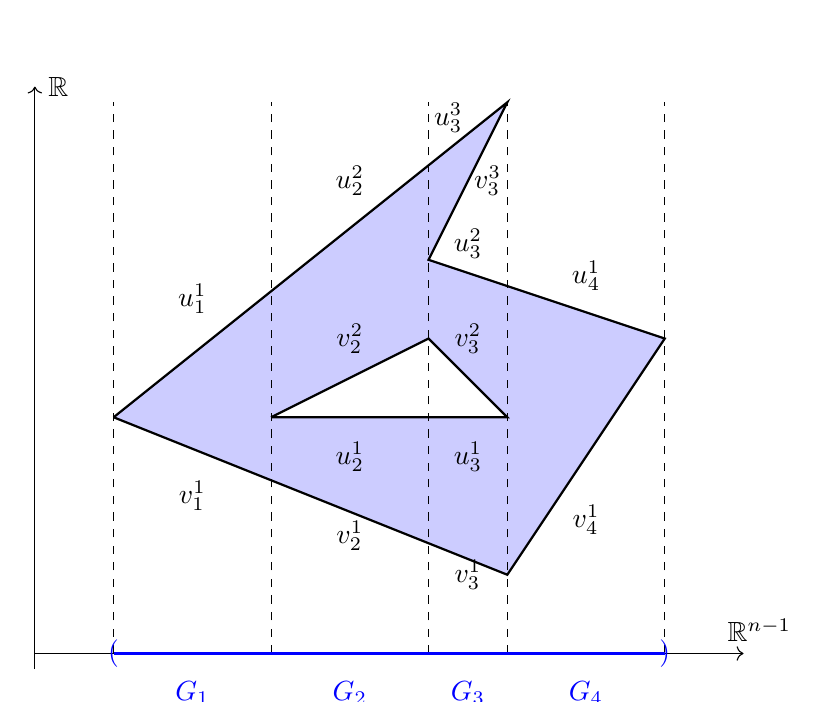
\begin{tikzpicture}
		%\draw[help lines] (-3,-3) grid (5,4);
        \draw [->](-4,-3) -- (5,-3);
        \node at (5.2,-2.7){\(\R^{n-1}\)};
        \draw [->](-4,-3.2) -- (-4,4.2);
        \node at (-3.7,4.2){\(\R\)};

        \fill[blue, opacity=0.2] (-3,0) -- (2,4)--(1,2)--(4,1)--(2,-2)--(-3,0);
        \draw[thick] (-3,0) -- (2,4)--(1,2)--(4,1)--(2,-2)--(-3,0);
        \draw[thick, fill=white] (-1,0)--(1,1)--(2,0)--(-1,0);
        \draw[dashed] (-3,-3)--(-3,4);
        \draw[dashed] (-1,-3)--(-1,4);
        \draw[dashed] (1,-3)--(1,4);
        \draw[dashed] (2,-3)--(2,4);
        \draw[dashed] (4,-3)--(4,4);
        
        \draw[thick, blue] (-3,-3)--(4,-3);
        \node[blue] at (-3,-3){\((\)};
        \node[blue] at (4,-3){\()\)};
        \node[blue] at (-2,-3.5){\(G_1\)};
        \node[blue] at (0,-3.5){\(G_2\)};
        \node[blue] at (1.5,-3.5){\(G_3\)};
        \node[blue] at (3,-3.5){\(G_4\)};

        \node at (-2,-1){\(v_1^1\)};
        \node at (-2,1.5){\(u_1^1\)};

        \node at (0,-1.5){\(v_2^1\)};
        \node at (0,-0.5){\(u_2^1\)};
        \node at (0,1){\(v_2^2\)};
        \node at (0,3){\(u_2^2\)};
    
        \node at (1.5,-2){\(v_3^1\)};
        \node at (1.5,-0.5){\(u_3^1\)};
        \node at (1.5,1){\(v_3^2\)};
        \node at (1.5,2.2){\(u_3^2\)};
        \node at (1.75,3){\(v_3^3\)};
        \node at (1.25,3.8){\(u_3^3\)};

        \node at (3,-1.3){\(v_4^1\)};
        \node at (3,1.8){\(u_4^1\)};
        
		\end{tikzpicture}
        \caption{Notation in step 1 of the proof of Theorem~\ref{thm: steiner inequality}.}
        \label{fig: polyhedral set}
	\end{figure}
    
    With this notation,
    \begin{equation}\label{eq: polyhedral perimeter}
    \begin{aligned}
        P(E) &= \Haus^{n-1}(\de E) = \sum_{h=1}^M\Haus^{n-1}(\de E \cap G_h \times \R) \\
        &= \sum_{h=1}^M \int_{G_h}\sum_{k=1}^{N(h)} \left( \sqrt{1+ |\nabla v_h^k|^2} + \sqrt{1+ |\nabla u_h^k|^2} \right)\dif z.
    \end{aligned}
    \end{equation}    
    For every \(z \in \R^{n-1}\),
    \[
        E_z = \left\{\begin{aligned}
            &\bigcup_{k=1}^{N(h)}(v_h^k(z), u_h^k(z))&& \text{ if }z \in G_h,\\
            &\ \varnothing &&\text{ if }z \in \R^{n-1}\setminus G
        \end{aligned} \right.
    \]
    and, if we set \(m(z)=\Leb^1(E_z)\) for every \(z \in \R^{n-1}\),
    \begin{equation}\label{eq: m(z)}
        m(z) \coloneq \Leb^1(E_z) = \left\{\begin{aligned} 
        & \sum_{k=1}^{N(h)} u_h^k(z)-v_h^k(z) && \text{ if }z \in G_h,\\
        & \ 0 &&\text{ if }z \in \R^{n-1}\setminus G.
        \end{aligned} \right.
    \end{equation}
    Observe that \(m \colon \R^{n-1} \to \R\) is affine on each \(G_h\). Therefore,
    \[
        E^s = \{ (z,t) \in \R^{n-1}\times \R \colon |t| < m(z)/2\}
    \]
    is a bounded set with polyhedral boundary, so in particular it has finite perimeter and \(|D\chi_{E^s}|= \Haus^{n-1}\resmes \de E^s\). By the area formula,
    \begin{equation}\label{eq: symmetrized polyhedral perimeter}
    \begin{aligned}
        P(E^s) &= \Haus^{n-1}(\de E^s) = 2 \int_G \sqrt{1+ \left|\frac{1}{2} \nabla m \right|^2} \dif z \\
        &= \sum_{h=1}^M\int_{G_h} \sqrt{4+ |\nabla m|^2} \dif z
    \end{aligned}
    \end{equation}

    By \eqref{eq: m(z)} and the convexity of the function \(z \mapsto \sqrt{1+|z|^2}\), for every \(h=1,\dots, M\)
    \begin{align*}
        \sum_{k=1}^{N(h)} \sqrt{1+|\nabla v_h^k|^2} + \sqrt{1+|\nabla u_h^k|^2} &\ge 2\sum_{k=1}^{N(h)} \sqrt{ 1+ \left|\frac{\nabla u_h^k-\nabla v_h^k}{2}\right|^2} \\
        &= 2N(h)\sum_{k=1}^{N(h)} \frac{1}{N(h)} \sqrt{ 1+ \left|\frac{\nabla u_h^k-\nabla v_h^k}{2}\right|^2}\\
        &\ge 2N(h) \sqrt{ 1+ \left|\sum_{k=1}^{N(h)} \frac{1}{N(h)}\frac{\nabla u_h^k-\nabla v_h^k}{2}\right|^2}\\
        &= \sqrt{4N(h)^2+|\nabla m|^2}.
    \end{align*}
    Therefore, by \(\eqref{eq: polyhedral perimeter}\) and \(\eqref{eq: symmetrized polyhedral perimeter}\), 
    \begin{equation}\label{eq: P(E^s)<(int)<P(E)}
        P(E^s) \le \sum_{k=1}^{N(h)} \int_{G_h} \sqrt{4N(h)^2+|\nabla m|^2} \dif z \le P(E).
    \end{equation}

    We have just found that
    \begin{align*}
        P(E)-P(E^s) &\ge \sum_{N(h)\ge 2} \int_{G_h} \left(\sqrt{4N(h)^2+|\nabla m|^2} - \sqrt{4+|\nabla m|^2} \right)\dif z\\
        &= \sum_{N(h)\ge 2} \int_{G_h} \frac{4(N(h)^2-1)}{\sqrt{4N(h)^2+|\nabla m|^2} + \sqrt{4+|\nabla m|^2}}\dif z\\
        & \ge \sum_{N(h)\ge 2} \int_{G_h} 2 \frac{1}{\sqrt{4N(h)^2 + |\nabla m|^2}} \dif z.
    \end{align*}
    If
    \[
        D \coloneq \{ z \in \R^{n-1} \colon E_z \text{ is not an interval}\} = \bigcup_{N(h)\ge 2} G_h,
    \]
    then by Cauchy-Schwarz inequality and \eqref{eq: P(E^s)<(int)<P(E)},
    \begin{equation}\label{eq: estimate on D}
        \begin{aligned}
            2\Leb^{n-1}(D)^2 &= 2 \left( \sum_{N(h)\ge 2}\int_{G_h} \frac{(4N(h)^2+|\nabla m|^2)^{1/4}}{(4N(h)^2+|\nabla m|^2)^{1/4}} \right)^2 \\
            &\le P(E) (P(E)-P(E^s)).
        \end{aligned}
    \end{equation}
    
    \emph{Step 2}. Now let \(E \subset \R^n\) with \(|E|<\infty\) and \(P(E)<\infty\). By Theorem~\ref{thm: polyhedral approximation} there exists a sequence of bounded sets \(E_h\) with polyhedral boundary such that
    \[
        E_h \to E, \qquad P(E_h) \to P(E).
    \]
    Note that we can assume that the outer unit normal of \(\de E_h\) is never orthogonal to \(e_n\). Indeed, this is an ‘‘open condition'', so if it happens that the unit normal of \(\de E_h\) is orthogonal to \(e_n\), we only need to rotate slightly \(\de E\). Doing smaller and smaller rotations as \(h \to \infty\), we still have that \(E_h \to E\) (while \(P(E_h) \to P(E)\) isn't affected by rotations). 

    For every \(h \in \N\), denote
    \[
        \begin{aligned}
            m_h(z) &\coloneq \Leb^1((E_h)_z), \quad m(z) \coloneq \Leb^1(E_z) \qquad \forall z \in \R^{n-1}\\
            G_h &\coloneq \{ z \in \R^{n-1} \colon m_h(z)>0\}, \qquad G\coloneq \{ z \in \R^{n-1} \colon m(z)>0\}\\
            D_h &\coloneq \{ z \in \R^{n-1} \colon (E_h)_z \text{ is not an interval}\}.
        \end{aligned}
    \]
    Applying step 1 to each \(E_h\), by \eqref{eq: P(E^s)<(int)<P(E)} and \eqref{eq: estimate on D} we get
    \begin{equation}\label{eq: step 1 to E_h}
        P(E_h^s) \le P(E_h), \qquad 2 \Leb^{n-1}(D_h)^2 \le P(E_h)(P(E_h)-P(E_h^s)).
    \end{equation}
    Moreover, by Fubini's theorem,
    \begin{equation*}
    \begin{aligned}
        |E\triangle E_h| &= \int_{\R^{n-1}} \Leb^1((E_h)_z \triangle E_z) \dif z \\
        &\ge \int_{\R^{n-1}}|m_h(z)- m(z)| \dif z = |E_h^s \triangle E^s|,
    \end{aligned}
    \end{equation*}
    so in particular \(E_h^s \to E^s\) and by lower semicontinuity
    \[
        P(E^s) \le \liminf_{h \to \infty} P(E_h^s) \le \lim_{h \to \infty} P(E_h) = P(E).
    \]
    Moreover,
    \begin{equation}\label{eq: G_h -> G, E_hz -> E_z}
        G_h \to G, \qquad (E_h)_z \to E_z \quad \text{ for a.e. }z \in \R^{n-1}
    \end{equation}
    By Proposition~\ref{prop: slicing} the vertical \(z\)-slices \((E_h)_z\) and \(E_z\) have finite perimeter for a.e. \(z \in \R^{n-1}\), thus by the lower semicontinuity of the perimeter
    \begin{equation}\label{eq: P(E_z) < liminf P(E_hz)}
        P(E_z) \le \liminf_{h \to \infty}P((E_h)_z).
    \end{equation}

    Now, assume that \(P(E)=P(E^s)\). Then, by \eqref{eq: step 1 to E_h}, \(\chi_{D_h} \to 0\) in \(L^1(\R^{n-1})\), so, up to passing to a subsequence, we have the pointwise limit
    \[
        \chi_{G}(z) = \lim_{h \to \infty}\chi_{G_h\setminus D_h}(z)
    \]
    for a.e. \(z \in \R^{n-1}\). By \eqref{eq: P(E_z) < liminf P(E_hz)},
    \[
        \chi_G(z)P(E_z) \le \liminf \chi_{G_h \setminus D_h}(z)P((E_h)_z) \qquad \text{ for a.e. } z \in \R^{n-1},
    \]
    therefore, by Fatou's lemma,
    \begin{equation*}
    \begin{aligned}
        \int_G P(E_z) \dif z & \le \int_{\R^{n-1}} \liminf \chi_{G_h \setminus D_h}(z)P((E_h)_z) \dif z\\
        &\le \liminf_{h \to \infty} \int_{G_h \setminus D_h}P((E_h)_z) \dif z\\
        &= 2 \liminf_{h \to \infty} \Leb^{n-1}(G_h \setminus D_h) \\
        &= 2 \Leb^{n-1}(G) \\
        &\le \int_G P(E_z) \dif z
    \end{aligned}
    \end{equation*}
    having used the 1-dimensional isoperimetric inequality in the last line, i.e., that \(P(E_z) \ge 2\) for a.e. \(z \in \R^{n-1}\). This implies that \(P(E_z)=2\) for a.e. \(z \in \R^{n-1}\), so, by the characterization of the equality in the 1-dimensional case, \(E_z\) is an interval for a.e. \(z \in \R^{n-1}\). 
\end{proof}

\begin{lemma}
    Let \(E\subset \R^n\) be a convex set with \(|E|<\infty\) and \(P(E)<\infty\), and let \(v\in\R^{n-1}\) a unit vector such that \(P(S_v(E))=P(E)\). Then there exists \(c \in \R\) such that \(E\) is equivalent to the translated \(S_v(E) + cv\).
\end{lemma}
\begin{proof}
    Assume without loss of generality that \(v=e_n\), and denote \(S_v(E)=E^s\). Since \(\Leb^n(\de E)=0\)\footnote{
    Indeed, without loss of generality assume that \(0 \in \mathring{C}\). Then by convexity, for every \(\eps>0\)
    \[  
        \de C \subset \left(\frac{1}{1-\eps}\mathring{C} \right) \setminus C.
    \]
    }, 
    we may assume that \(E\) is open. Then the projection \(G\subset \R^{n-1}\) is a convex set, and for every \(z \in G\), the vertical \(z\)-slice is equivalent to the open interval \((-v(z),u(z))\), where \(v,u \colon G \to \R\) are concave non negative functions, so in particular they are locally Lipschitz and \(E\) has Lipschitz boundary. By Rademacher's theorem, \(\nabla u\) and \(\nabla v\) are defined at a.e. \(z \in G\), so
    \begin{equation*}%\label{eq: P(E), P(E^s) convex case}
    \begin{aligned}
        P(E) &= \int_G \left( \sqrt{1+|\nabla u|^2} + \sqrt{1+|\nabla v|^2} \right) \dif z\\
        P(E^s) &= 2\int_G  \sqrt{1+\left| \frac{\nabla u + \nabla v}{2}\right|^2} \dif z
    \end{aligned}
    \end{equation*}
    since 
    \[  
        E^s = \left\{ (z,t) \in G \times \R \colon |t|< \frac{u(z)+v(z)}{2}\right\}.
    \]
    By the strict convexity of the function \(z \mapsto \sqrt{1+|z|^2}\),
    \[
        \sqrt{1+|\nabla u|^2} + \sqrt{1+|\nabla v|^2} \ge 2\sqrt{1+\left| \frac{\nabla u + \nabla v}{2}\right|^2}
    \]
    with equality if and only if \(\nabla u = \nabla v\). Hence, if \(P(E^s)=P(E)\), the equality holds almost everywhere and there must be that \(\nabla u = \nabla v\) a.e. in \(G\). Thus, there exists \(c \in \R\) such that \(u(z)-v(z)= c\) for a.e. \(z \in G\), which implies that 
    \[
    \begin{aligned}
        E&= \left\{ (z,t) \in G \times \R \colon -u(z)-c < t < u(z)\right\},\\
        E^s&= \left\{ (z,t) \in G \times \R \colon -u(z)-c/2 < t < u(z)+c/2\right\},
    \end{aligned}
    \]
    that is \(E= E^s + \frac{c}{2}e_n\).
\end{proof}

Recall that the density of \(E\) at a point \(x \in \R^n\) is
\[
    \Theta(E,x) \coloneq \lim_{r \to 0} \frac{|E \cap B_r(x)|}{\omega_n r^n}
\]
whenever it exists. It's easy to show that, whenever this limit exists, it's actually equal to
\begin{equation}\label{eq: density with cubes}
    \Theta(E,x)= \lim_{r \to 0} \frac{|E \cap Q^n(x,r)|}{2^nr^n}
\end{equation}
where
\[
    Q^n(x,r)= x+(-r,r)^n
\]
is the cube centered at \(x\) with side \(2r\). 

Observe that \(\Leb^n \resmes E= \chi_E \Leb^n\), so by Besicovitch differentiation theorem, 
\[
    \chi_E = \frac{\dif (\Leb^n \resmes E)}{\dif \Leb^n} = \Theta(E,\cdot)
\]
a.e. on \(\R^n\), that is,
\[
    \Theta(E,x)= \begin{cases}
        1 & \text{ a.e. }x \in E\\
        0 & \text{ a.e. }x \in \R^n \setminus E.
    \end{cases}
\]
In particular, \(E\) is equivalent to
\[
    E^{(1)} \coloneq \{ x \in \R^n \colon \Theta(E,x)=1\},
\]
the set of with density one points of \(E\). This will be the ‘‘good set'' to replace \(E\) with.

\begin{lemma}\label{lemma: density points and vertical sections}
    Let \(E \subset \R^n\) be a set of locally finite perimeter and suppose that \(E_z\) is equivalent to an interval for a.e. \(z \in \R^{n-1}\). Then \((E^{(1)})_z\) is an interval for every \(z \in \R^{n-1}\).
\end{lemma}
\begin{proof}
    Let \(z_0 \in \R^{n-1}\), and suppose that \(x_1=(z_0,t_1),x_2=(z_0,t_2) \in E^{(1)}\) for some \(t_1<t_2\), and fix \(t_0 \in (a,b)\). We have to prove that \(x_0=(z_0,t_0) \in E^{(1)}\), that is \(\Theta(E,x_0)=1\).

    Fix \(0<\eps< 1\), and for every \(t \in \R\), \(r>0\) denote \(I_r(t) = B_r(t)= (t-r,t+r)\). Since \(x_1,x_2 \in E^{(1)}\), \(\Theta(E,x)=\Theta(E,y)=1\), so by \eqref{eq: density with cubes} there exists \(\overline{r}>0\) such that for every \(r<\overline{r}\)
    \begin{equation}\label{eq: x_k density one}
        |E\cap Q^n(x_k,r)| \ge \left(1-\frac{\eps}{2}\right) 2^n r^n, \quad I_r(t_0)\cap I_r(t_k)=\varnothing \qquad k=1,2.
    \end{equation}
    Fix \(r<\overline{r}\) and for \(k=1,2\) denote by \(G_k\) the set of \(z \in Q^{n-1}(z_0,r)\) such that \(E_z\) is equivalent to an interval and \(\Leb^1(E_z \cap I_r(t_k))>0\). Since \(E_z\) is equivalent to an interval for a.e. \(z \in \R^{n-1}\), by Fubini's theorem
    \[
        |E \cap Q^n(x_k,r)| = \int_{G_k} \Leb^1(E_z \cap I_r(t_k)) \dif z \le 2r \Leb^{n-1}(G_k).
    \]
    Combining this with \eqref{eq: x_k density one},
    \[
        \Leb^{n-1}(G_k) \ge \left(1-\frac{\eps}{2}\right) 2^{n-1} r^{n-1}, \qquad k=1,2.
    \]
    Therefore, 
    \[
    \begin{aligned}
        \Leb^{n-1}(G_1\cap G_2) &= \Leb^{n-1}(G_1) +\Leb^{n-1}(G_2) - \Leb^{n-1}(G_1 \cup G_2) \\
        &\ge \Leb^{n-1}(G_1) +\Leb^{n-1}(G_2) - \Leb^{n-1}(Q^{n-1}(z_0,r))\\
        &\ge (1-\eps) 2^{n-1} r^{n-1}.
    \end{aligned}        
    \]
    Now let \(z \in G_1 \cap G_2\). Since \(E_z\) is equivalent to an interval and \(\Leb^1(E_z \cap I_r(t_k))>0\) for \(k=1,2\), by \eqref{eq: x_k density one} we have
    \[
        \Leb^1(E_z \cap I_r(t_0))=2r.
    \]
    Integrating this over \(G_1 \cap G_2\), we find
    \[
    \begin{aligned}
        |E\cap Q^n(x_0,r)| &\ge \int_{G_1\cap G_2} \Leb^1(E_z \cap I_r(t_0)) \dif z \\
        &= 2r \Leb^{n-1}(G_1 \cap G_2) \ge (1-\eps) 2^n r^n.
    \end{aligned}
    \]
    for every \(r<\overline{r}\). Since \(\eps>0\) was arbitrary,
    \[
        \lim_{r \to 0} \frac{|E\cap Q^n(x_0,r)|}{2^n r^n} = 1,
    \]
    which proves that \(x_0 \in E^{(1)}\). 
\end{proof}

\section{The isoperimetric inequality}
\begin{lemma}[Constrained isoperimetric inequality]\label{lemma: constrained isoperimetric inequality}
    Let \(m,R>0\) with \(m<\omega_nR^n\). Then 
    \[
        \alpha(m,R) \coloneq \inf\{ P(E) \colon E \subset B_R \text{ measurable, } |E|=m\}
    \]
    is realized, and every minimizer is equivalent to a ball. In particular, \(\alpha(m,R)\) is the perimeter of a ball of volume \(m\), that is
    \[
        \alpha(m,R) = n \omega_n^{1/n} m^{\frac{n-1}{n}}.
    \]
\end{lemma}
\begin{proof}
    That \(\alpha(m,R)\) is realized is a consequence of the Direct Method, as bounded sets in \(BV(B_R)\) are precompact with respect to the BV-strict convergence, the family of characteristic functions of sets in \(B_R\) is closed, and any limit in the class preserves the volume. 

    Let us now assume that \(E \subset B_R\) satisfies \(|E|=m\) and \(P(E)=\alpha(m,R)\). Since \(|E\triangle E^{(1)}|=0\), we may assume that \(E=E^{(1)}\). For every unit vector \(v \in \R^n\), \(|v|=1\), by Theorem~\ref{thm: steiner inequality} we have that \(P(S_v(E))\le P(E)\). On the other hand, by the properties of the Steiner symmetrization \(|S_v(E)|=m\) and \(\diam(S_v(E)) \le \diam E<R\), so \(P(S_v(E)) \ge \alpha(m,R)=P(E)\). Then by Theorem~\ref{thm: steiner inequality} and Lemma~\ref{lemma: density points and vertical sections} 
    \[
        E_{v,z} \coloneq \{ s \in \R \colon z + sv \in E\}
    \]
    is an interval for every \(z \in v^\perp\). 

    We claim that \(E\) is convex. Indeed, let \(x,y \in E\) be two distinct points, and set \(v = (y-x)/|y-x|\). Then if \(z \in v^\perp\) is the projection of \(x\) (and \(y\)) in \(v^\perp\), 
    \[
        (1-\lambda)x + \lambda y = z + [(1-\lambda)x\cdot v + \lambda x \cdot v] v \in E, \qquad \forall \lambda \in [0,1]
    \]
    as \([x\cdot v, y\cdot v] \subset E_{v,z}\).

    By Theorem~\ref{thm: steiner inequality}, for every unit vector \(v \in \R^n\) there exists \(c_v \in \R\) such that \(E= S_v(E) + c_v v\). Consider
    \[
        E' \coloneq E - (c_{e_1}e_1 + \cdots c_{e_n}e_n).
    \]
    Since \(E'\) is still convex and for every unit vector \(v \in \R^n\) we still have \(P(E')=P(S_v(E'))\), there are constants \(c_v' \in \R\) such that \(E' = S_v(E')+c_v'v\). But by construction, 
    \[
        S_{e_i}(E') = S_{e_i}(E) - \sum_{j \ne i} c_j e_j = E-c_ie_i - \sum_{j \ne i} c_j e_j = E',
    \]
    so \(c_i'=0\) for every \(i=1,\dots,n\). Hence, \(E'\) is invariant under the reflections with respect to the coordinates planes, and therefore invariant under the map \(x\mapsto -x\) (the composition of all those reflections). Since for every unit vector \(v\) we can write \(E'=S_v(E)+c_v'v\), we have
    \begin{equation}\label{eq: gaining symmetry}
        S_v(E)+c'_vv =  -S_v(E) - c'_vv = S_v(E) + c'_v(-v).
    \end{equation}
    Clearly, \(c_{-v}'=-c_v'\) for every unit vector \(v\). On the other hand, combining \eqref{eq: gaining symmetry} with the fact that \(S_v(E)=S_{v'}(E)\), we also have that \(c_v'=c_{-v}'\). Therefore, for every unit vector \(v \in \R^n\), it must be \(c_v'=0\), that is, \(S_v(E')=E'\).
    
    As a consequence, \(E'\) is invariant under reflections by hyperplanes through the origin. Since by composition the set of those reflections generates all rotations that fix the origin, \(E'\) is invariant under any rotation fixing the origin. As a consequence, all the sections 
    \[
        E_v' \coloneq  \{ s \in \R \colon sv \in E'\}, \qquad v\in \R^n, \ |v|=1,
    \]
    must be equal, and since \(E'\) is bounded there exists \(r>0\) such that \(E_v'=(-r,r)\) for every unit vector \(v \in \R^n\). Hence, \(E'=B_r(0)\) and \(E=B_r(p)\), with \(p=(c_{e_1},\dots,c_{e_n})\).
\end{proof}

We can now prove the isoperimetric inequality.
\begin{proof}[Proof of Theorem~\ref{thm: isoperimetric inequality}]
    Suppose that \(E\) is bounded. Then taking \(R>0\) big enough, by Lemma~\ref{lemma: constrained isoperimetric inequality}, 
    \[
        P(E) \ge n \omega_n^{1/n} |E|^{\frac{n-1}{n}},
    \]
    and the equality holds if and only if \(E\) is equivalent to a ball.

    If \(E\) is not bounded, by Theorem~\ref{thm: polyhedral approximation} we can approximate it with bounded sets, that is, there are bounded sets \(E_h\subset \R^n\) with \(E_h \to E\) and \(P(E_h) \to P(E)\). Passing to the limit, the inequality is preserved. 
    
    Now assume that \(E=E^{(1)}\) is unbounded and \(|E|<\infty\). Assume by contradiction that 
    \[
        P(E) = n \omega_n^{1/n} |E|^{\frac{n-1}{n}}.
    \]
    By \eqref{thm: steiner inequality}, \(P(E)=P(S_v(E))\) for every unit vector \(v \in \R^n\). Up to a translation, arguing exactly as in Lemma~\ref{lemma: constrained isoperimetric inequality} we have that all the sections \(E\)
    \[
        E_v \coloneq  \{ s \in \R \colon sv \in E\}, \qquad v\in \R^n, \ |v|=1,
    \]
    are equal. Since \(E\) is unbounded, we have \(E_v=\R\) for every unit vector \(v \in \R^n\), but then \(E=\R^n\), a contradiction in because we assumed that \(|E|<\infty\).
\end{proof}




\section{An alternative approach}
Adopting the point of view of differential geometry, we could have used a completely different approach. Indeed, fix \(m>0\) and let
\begin{equation}\label{eq: isoperimetric problem}
    \alpha(m) \coloneq \inf\left\{ \Haus^{n-1}(\Sigma) \left| \ \begin{aligned}
        &\Sigma = \de \Omega \text{ smooth, connected,}\\
        &\text{compact hypersurface}, |\Omega|=m
    \end{aligned}
    \right.\right\}.
\end{equation}
Suppose that \(\Sigma= \de \Omega\) is a minimizer, that is, \(\Haus^{n-1}(\Sigma) = \alpha(m)\) and \(|\Omega|=m\). Let \(\nu \colon \Sigma \to \Sp^{n-1}\) be the outer unit normal of \(\Sigma\), \(A\) its second fundamental form, defined\footnote{
Note that, identifying the tangent spaces as subspaces of \(\R^n\) in the usual way, the scalar product makes sense. Actually, \(T_{\nu(x)} \Sp^{n-1}=T_x\Sigma \subset \R^n\) by definition of unit normal.
} by 
\[
    A(X,Y)=\dif \nu_x [X] \cdot Y
\]
for every tangent vectors \(X,Y \in T_x \Sigma\), and \(H = \tr(A)\) its mean curvature. By the inverse function theorem and by the compactness of \(\Sigma\), there is \(\eps>0\) such that 
\[
    \phi(t,x) = x + t\nu(x),
\]
is a diffeomorphism on \((-\eps,\eps) \times \Sigma\). Let \(u\colon \Sigma \to \R\) be a smooth function with zero average, i.e., \(\int_\Sigma u \dif \Haus^{n-1}=0\), and define
\[
    F(t,x) = \phi(tu(x),x)
\]
for every \(x \in \Sigma\) and \(t \in \R\) small enough. Denote 
\[
    \Sigma_t = \{F(t,x) \colon x \in \Sigma\}.
\]
Then, \(\Sigma_t = \de \Omega_t\) is the boundary of a bounded set \(\Omega_t\). For every \(x \in \Sigma\), consider the geodesic
\[
    \gamma_x(s) = \phi(s,x),
\]
which has constant velocity \(|\dot \gamma_x|=u(x)\). Then, by the coarea formula,
\[
\begin{aligned}
    |\Omega_t| &= |\Omega| + |\{ \phi(s,x) \colon 0<s<tu(x)\}| - |\{ \phi(s,x) \colon tu(x)<s<0\}| \\
    &= m+ \int_{\{u>0\}} \int_0^t |\dot \gamma_x| \dif t  \dif \Haus^{n-1}(x) - \int_{\{u<0\}} \int_0^t |\dot \gamma_x| \dif t \dif \Haus^{n-1}(x)\\
    &= m + t\int_\Sigma u \ \dif \Haus^{n-1} = m,
\end{aligned}
\]
hence \(\Sigma_t\) is a competitor in \eqref{eq: isoperimetric problem} for every \(t\). By the minimality of \(\Sigma\),
\[
    \Haus^{n-1}(\Sigma_t) \ge \Haus^{n-1}(\Sigma),
\]
so the function \(t \mapsto \Haus^{n-1}(\Sigma_t)\) has a minimum at \(t=0\). The first variation formula implies that
\[
   0 = \left.\frac{\dif}{\dif t}\right|_{t=0} \Haus^{n-1}(\Sigma_t) = \int_\Sigma Hu \ \dif \Haus^{n-1}.
\]
Since this hold for every \(u:\Sigma \to \R\) with zero average, \(H\) is constant, and we say that \(\Sigma\) is \emph{CMC}.

Taking the second derivative with respect to \(t\), the second variation formula implies that
\begin{equation}\label{eq: stability inequality}
\begin{aligned}
    0 &\le \int_\Sigma |\nabla_\Sigma u|^2 - (|A|^2-H^2) u^2  \ \dif \Haus^{n-1} \\
    &= \int_\Sigma |\nabla_\Sigma u|^2 - |A|^2 u^2 \ \dif \Haus^{n-1}= - \int_\Sigma u L_\Sigma u \ \dif \Haus^{n-1}
\end{aligned}
\end{equation}
for every smooth function \(u\) with zero average, where 
\[
    L_\Sigma u = \Delta_\Sigma u + |A|^2u
\]
is the \emph{Jacobi operator} of \(\Sigma\). Any hypersurface \(\Sigma\) that satisfies \eqref{eq: stability inequality} is called \emph{CMC-stable}. 

This approach can give another proof of the isoperimetric inequality. In particular, it holds the following stronger result.

\begin{thm}[Barbosa-do Carmo, {\cite{BarbosaDoCarmo}}]\label{thm: Barbosa-do Carmo}
    Let \(\Sigma\) be a compact, connected, orientable, CMC hypersurface in \(\R^n\). Then \(\Sigma\) is CMC-stable if and only if \(\Sigma\) is a round sphere.
\end{thm}

\begin{proof}
Let \(\Sigma\) be a sphere, and assume without loss of generality that \(\Sigma = \Sp^{n-1}\) has radius \(1\) and is centered at the origin. Since \(\nu(x)=x\), we have \(\dif \nu = \id\), hence \(H = (n-1)\) and \(|A|^2 = (n-1)\). Thus, \(\Sp^{n-1}\) is CMC. The spectrum of the spherical Laplacian \(\Delta_{\Sp^{n-1}}\) is well known thanks to the formula of the standard Laplacian of \(\R^n\) in spherical coordinates
\[
    \Delta_{\R^n} = \frac{\de^2}{\de r^2} + \frac{n-1}{r} \frac{\de}{\de r} + \frac{1}{r^2}\Delta_{\Sp^{n-1}},
\]
that allows us to identify the homogeneous harmonic functions of \(\R^n\) with the eigenfunctions of \(\Delta_{\Sp^{n-1}}\). In particular, the first nonzero eigenvalue of \(\Delta_{\Sp^{n-1}}\) is
\[
\begin{aligned}
    \lambda_1 &= \inf\left\{ \frac{\int_{\Sp^{n-1}} |\nabla_{\Sp^{n-1}} u|^2  \dif \Haus^{n-1}}{\int_{\Sp^{n-1}} u^2 \dif \Haus^{n-1}} \colon u \in C^{\infty}(\Sp^{n-1}) \setminus \{0\},\ \int_{\Sp^2} u \ \dif \Haus^{n-1}=0\right\} \\
    &=(n-1).
\end{aligned}
\]
Thus, for every smooth function \(u \colon \Sp^{n-1} \to \R\) with zero average
\[
    \int_{\Sp^{n-1}} |\nabla_{\Sp^{n-1}}u|^2-(n-1)u^2 \ \dif \Haus^{n-1} \ge 0,
\]
that is, \(\Sp^{n-1}\) is CMC-stable.

Now assume that \(\Sigma\) is CMC-stable, and let us prove that it must be a sphere.
Consider the function \(f \colon \Sigma \to \R\) defined by
\[
    f(x)= x \cdot \nu(x) 
\]
and the radial vector field \(X(x)=x\), for every \(x \in \Sigma\). Even if \(X\) is not tangent, we can define its divergence on \(\Sigma\) as
\[
    \dive_\Sigma X = \sum_{i=1}^{n-1} (D_{\tau_i} X) \cdot \tau_i 
\]
locally for any orthonormal frame \(\tau_1,\dots,\tau_n\) of \(\Sigma\). Since \(X\) is the restriction of the identity,
\[
    \dive_\Sigma X = \sum_{i=1}^{n-1} (D_{\tau_i} X) \cdot \tau_i = \sum_{i=1}^{n-1} \tau_i \cdot \tau_i = n-1.
\]
By the generalized divergence theorem for submanifolds,
\[  
\begin{aligned}
    \int_\Sigma \dive_\Sigma X \ \dif \Haus^{n-1} &= \int_{\de\Sigma} X \cdot \nu_{\de \Sigma} \ \dif \Haus^{n-2} + \int_\Sigma HX\cdot \nu \ \dif \Haus^{n-1}\\
    &= H\int_\Sigma f(x) \ \dif \Haus^{n-1}(x)
\end{aligned}
\]
because \(\de \Sigma = \varnothing\). Therefore, \(u = Hf-n+1\) has zero average, and can be tested in \eqref{eq: stability inequality}.

With a clever choice of frame, one can compute that
\begin{equation}\label{eq: Laplacian of f}
    \Delta_\Sigma f = H-|A|^2f.
\end{equation}
Therefore,
\[
    L_\Sigma u = H^2-|A|^2Hf + |A|^2(Hf-n+1) = H^2-(n-1)|A|^2,
\]
and \eqref{eq: stability inequality} becomes
\[
\begin{aligned}
    0 &\le \int_\Sigma ((n-1)|A|^2-H^2) (Hf-n+1) \ \dif \Haus^{n-1}\\
    &= (n-1)\int_\Sigma |A|^2(Hf-n+1) \ \dif \Haus^{n-1}.
\end{aligned}
\]
By the divergence theorem and by \eqref{eq: Laplacian of f}
\[
    0 = \int_\Sigma \Delta_\Sigma f \ \dif \Haus^{n-1} = H\Haus^{n-1}(\Sigma)- \int_{\Sigma} |A|^2 f \ \dif \Haus^{n-1},
\]
so 
\[
    0 \le \int_\Sigma |A|^2(Hf-n+1) \ \dif \Haus^{n-1} = \int_\Sigma H^2-(n-1)|A|^2 \dif \Haus^{n-1},
\]
that is
\begin{equation}\label{eq: (n-1)int |A|^2<int H^2}
    (n-1)\int_\Sigma |A|^2\dif \Haus^{n-1} \le \int_\Sigma H^2 \dif \Haus^{n-1}.
\end{equation}
However, if \(\lambda_1, \dots, \lambda_{n-1}\) are the eigenvalues of \(A\), by the \(AM\le QM\) inequality we have that
\[
    H^2 = \left(\sum_{i=1}^{n-1}\lambda_i\right)^2 \le (n-1)\sum_{i=1}^{n-1}\lambda_i^2 = (n-1) |A|^2,
\]
with equality if and only if \(\lambda_1= \cdots =\lambda_{n-1}\). But by \eqref{eq: (n-1)int |A|^2<int H^2}, it must be \(H^2=(n-1)|A|^2\), that is,
\[
    \dif \nu = \frac{H}{n-1} \id 
\]
(in this case, \(\Sigma\) is called \emph{totally umbilical}). This implies that \(\Sigma\) is a sphere. Indeed, consider the map \(F \colon \Sigma \to \R^n\) given by
\[
   F(x) = \frac{H}{n-1}x-\nu(x) 
\]
for every \(x \in \Sigma\). Its differential vanishes, so, since \(\Sigma\) is connected, it's constant: there exists \(p \in \R^n\) such that
\[
    F(x)=\frac{H}{n-1}p
\]
for every \(x \in \Sigma\). But then
\[
    \nu(x) = \frac{H}{n-1}(x-p),
\]
and therefore
\[
    |x-p|= \frac{n-1}{|H|},
\]
for every \(x \in \Sigma\), that is, \(\Sigma\) is the sphere of radius \((n-1)/|H|\) centered at \(p\).
\end{proof}

\printbibliography
\addcontentsline{toc}{section}{References}
\end{document}

